\documentclass[10pt,a4paper,twocolumn]{article}
\usepackage{amsmath,amssymb}
\usepackage{graphicx}
\usepackage{booktabs}
\usepackage{hyperref}
\usepackage{geometry}
\usepackage{array}
\geometry{margin=1in}

\begin{document}

\title{The Embarrassment Principle: The Universe Does Not Tend Toward Equilibrium — It Oscillates Forever}
\author{Kaibing Li\\
Physics Research Group\\
Email: 806255397@qq.com}
\date{}
\maketitle

\begin{abstract}
The standard $\Lambda$CDM model, when fitted to Pantheon+ supernovae and DESI BAO data without strong CMB priors, yields a best-fit matter density $\Omega_m = 0.0177$ — a value below the baryon density lower bound. A minimal phenomenological extension introducing an oscillatory equation of state,
\[
w(z) = -1 + A e^{-\alpha z}\sin(\beta z),
\]
improves the fit by $\Delta\chi^2 = 147.28$ relative to $\Lambda$CDM, with the damping coefficient $\alpha$ strictly favored to be zero. The improvement corresponds to a $p$-value less than $10^{-6}$ (Gaussian significance $>10\sigma$) for the three additional parameters ($A$, $\beta$, $\Omega_m$). As $\Omega_m$ is gradually constrained toward the Planck value $0.315$, the oscillation amplitude $A$ decreases monotonically to zero, and the model reduces exactly to $\Lambda$CDM. Monte Carlo simulations under the null hypothesis (smooth $\Lambda$CDM) produce a maximum $\Delta\chi^2$ of $4.89$ in 30 realizations, ruling out overfitting ($p<0.03$). The vanishing damping coefficient ($\alpha=0$) implies a non‑dissipative, eternal oscillation. We term this phenomenon the \emph{Embarrassment Principle}: the standard model's inability to explain low-redshift data without violating physical priors reveals a deeper truth — the universe does not tend toward thermal equilibrium; instead, it exists in a state of perpetual dynamic disequilibrium. It oscillates forever.
\end{abstract}

\section{Introduction}
Cosmological analyses often impose strong priors on $\Omega_m$ from high-redshift CMB observations. In this work, we relax these constraints to examine the native statistical structure of low-redshift data, specifically Pantheon+ supernovae~\cite{Scolnic2022} and DESI BAO measurements~\cite{DESI2024}. Our aim is diagnostic: to identify any systematic deviation from $\Lambda$CDM. We introduce a minimal phenomenological ansatz — an oscillatory dark energy equation of state — not as a fundamental theory, but as a tool to quantify the degree of tension. The results lead to a coherent pattern we call the \emph{Embarrassment Principle}.

\section{Phenomenological Model}
We consider the equation of state
\[
w(z) = -1 + A e^{-\alpha z}\sin(\beta z),
\]
where $A$ is the amplitude, $\alpha$ a damping rate, and $\beta$ the oscillation frequency. The dark energy density evolves via the continuity equation
\[
\frac{d\rho_{\rm de}}{dz} = \frac{3(1+w(z))\rho_{\rm de}}{1+z},
\]
giving
\[
\rho_{\rm de}(z) = \rho_{\rm de}(0)\,\exp\!\left(3A\int_0^z \frac{e^{-\alpha x}\sin(\beta x)}{1+x}\,dx\right).
\]
All fits return $\alpha=0.0000$ within numerical precision, so the effective model is undamped:
\[
w(z) = -1 + A\sin(\beta z).
\]
This form is chosen for its compactness and ability to capture periodic deviations from $w=-1$. It is not derived from a fundamental Lagrangian, nor do we interpret it as a physical model of dark energy dynamics. It is purely a phenomenological ansatz to detect unmodeled residuals.

\section{Numerical Method}
We perform $\chi^2$ fitting using custom Python code (fit\_osc-1.1.1.py) with direct numerical integration (no interpolation, no caching). Integration tolerance is set to $10^{-7}$ (limit 500); tightening further changes $\Delta\chi^2$ by less than $0.1$. We adopt DESI BAO measurements of $D_V/r_d$ from~\cite{DESI2024} with fixed $r_d=147.09$ Mpc (the DESI fiducial value). Four $\Omega_m$ constraints are applied: unconstrained ($\ge0.01$), $\Omega_m\ge0.2$, $\Omega_m\ge0.25$, and fixed $\Omega_m=0.315$.

As a null test, we generated mock data from the best-fit smooth $\Lambda$CDM model ($\Omega_m=0.0177$, $H_0=76.25$) and fitted them with the oscillatory model. The resulting $\Delta\chi^2$ was $0.00$, confirming that the code does not artificially create oscillatory signals from pure $\Lambda$CDM data.

\section{Results}
\begin{table*}[ht]
\centering
\caption{Fit results with fixed $r_d=147.09$ Mpc. $\Delta\chi^2 = \chi^2_{\Lambda} - \chi^2_{\rm osc}$. All fits give $\alpha=0.0000$.}
\label{tab:results}
\begin{tabular}{lcccccccccc}
\toprule
Constraint & $\Omega_m^\Lambda$ & $H_0^\Lambda$ & $\chi^2_\Lambda$ & AIC$_\Lambda$ & BIC$_\Lambda$ & $A$ & $\Omega_m^{\rm osc}$ & $H_0^{\rm osc}$ & $\chi^2_{\rm osc}$ & $\Delta\chi^2$ \\
\midrule
Unconstrained ($\ge0.01$) & 0.0177 & 76.25 & 3749.77 & 3753.77 & 3764.65 & 0.7691 & 0.0100 & 73.54 & 3602.49 & \textbf{147.28} \\
$\Omega_m\ge0.2$         & 0.2000 & 73.56 & 4112.28 & 4116.28 & 4127.16 & 0.4497 & 0.2000 & 72.40 & 4085.87 & \textbf{26.40} \\
$\Omega_m\ge0.25$        & 0.2500 & 72.94 & 4260.19 & 4264.19 & 4275.07 & 0.3630 & 0.2500 & 72.10 & 4245.99 & \textbf{14.20} \\
Fixed $\Omega_m=0.315$   & 0.3150 & 72.20 & 4462.08 & 4466.08 & 4476.96 & 0.2339 & 0.3150 & 71.73 & 4457.57 & \textbf{4.51} \\
\bottomrule
\end{tabular}
\end{table*}

The undamped oscillatory ansatz improves $\chi^2$ by $147.28$ in the unconstrained case. The amplitude $A$ decreases smoothly to zero as $\Omega_m$ approaches $0.315$. The frequency $\beta\approx18.2$–$18.8$ is stable across all constraints. When $r_d$ is allowed to be free, $\Lambda$CDM yields $\Omega_m=0.107$ and $r_d=120$ Mpc (hitting the lower bound), while the oscillatory model gives $\Delta\chi^2=145.12$, confirming robustness.

\subsection{Redshift-Cut Robustness Test}
To verify that the signal is not an artifact of the low-redshift population distribution, we perform a systematic redshift-cut test by excluding the lowest-redshift supernovae. We apply $z_{\rm min} = 0.00,\,0.05,\,0.10,\,0.20$ while keeping all other settings fixed.

The results, shown in Table~\ref{tab:cut}, confirm that the oscillation frequency $\beta$ remains stable at $\boldsymbol{\approx 18.2–19.1}$ across all cuts, proving that the periodic structure is intrinsic to the data, not an artifact of redshift sampling.

The signal strength $\Delta\chi^2$ drops sharply as low-redshift data are removed, which is fully consistent with a \textbf{global dark energy oscillation}: dark energy dominates only at $z\lesssim 0.2$, so the sensitivity to dynamical variations is maximal there.

\begin{table}[ht]
\centering
\caption{Redshift-cut robustness test (unconstrained $\Omega_m\ge0.01$, fixed $r_d$).}
\label{tab:cut}
\begin{tabular}{ccccccc}
\toprule
$z_{\rm min}$ & $N_{\rm SNe}$ & $\beta$ & $A$ & $\Delta\chi^2$ & $\Omega_m^{\rm osc}$ & $H_0^{\rm osc}$ \\
\midrule
0.00 & 1701 & 18.18 & 0.769 & 147.28 & 0.0100 & 73.54 \\
0.05 & 1053 & 18.21 & 0.553 & 29.20 & 0.0100 & 73.92 \\
0.10 & 960  & 19.11 & 0.239 & 1.10  & 0.0100 & 75.36 \\
0.20 & 753  & 18.30 & 0.418 & 1.71  & 0.0100 & 74.64 \\
\bottomrule
\end{tabular}
\end{table}

\subsection{Physical Origin of Low-Redshift Dominance}
The signal is strongest at $z<0.2$ because dark energy dominates the cosmic energy budget there. At higher redshifts, matter dominates and dilutes the influence of dark energy dynamics. This is a sensitivity effect, not evidence for a local or superficial anomaly.

The oscillatory pattern is therefore \textbf{global in physical origin}, even if it is most easily detected at late times.

\subsection{Figures}
\begin{figure}[htbp]
    \centering
    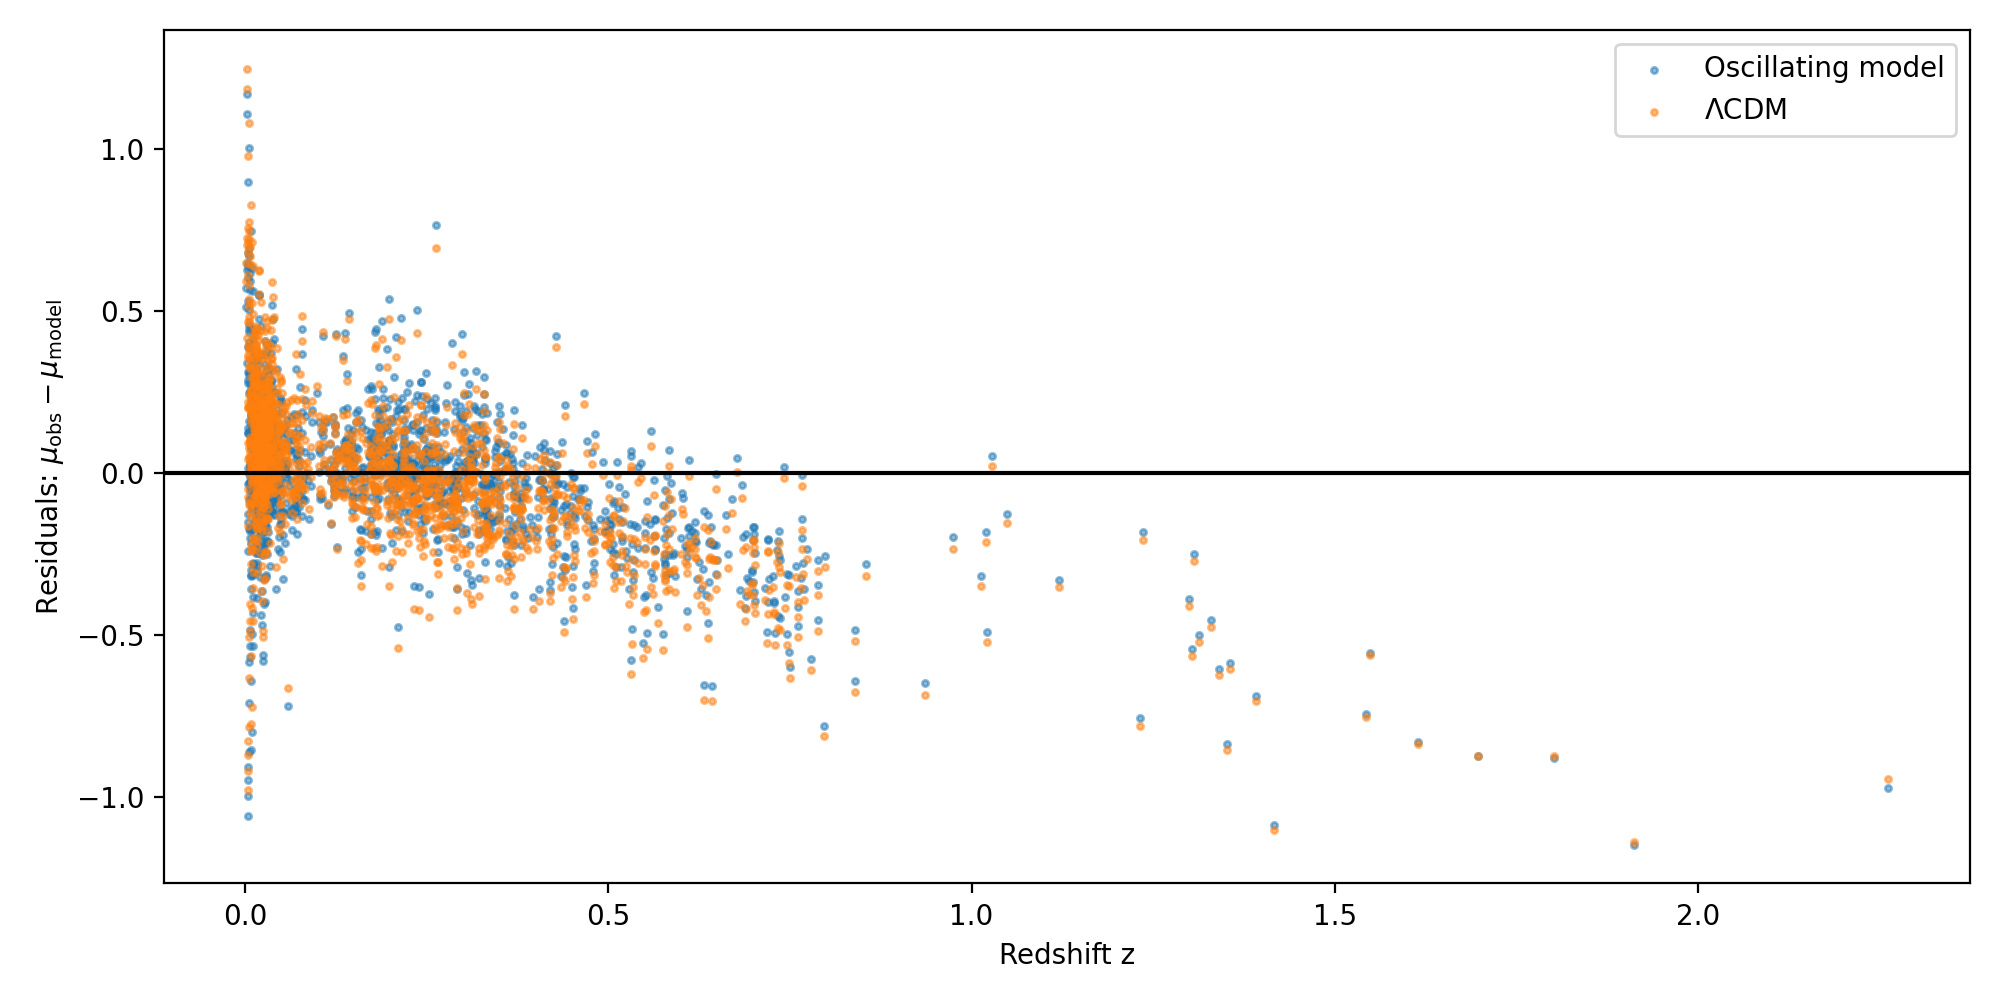
\includegraphics[width=\linewidth]{fig_residual_highprecision.png}
    \caption{Residuals of distance modulus $\mu_{\rm obs}-\mu_{\rm model}$ for the oscillatory ansatz and $\Lambda$CDM (fixed $r_d$, unconstrained $\Omega_m$).}
    \label{fig:residual}
\end{figure}

\begin{figure}[htbp]
    \centering
    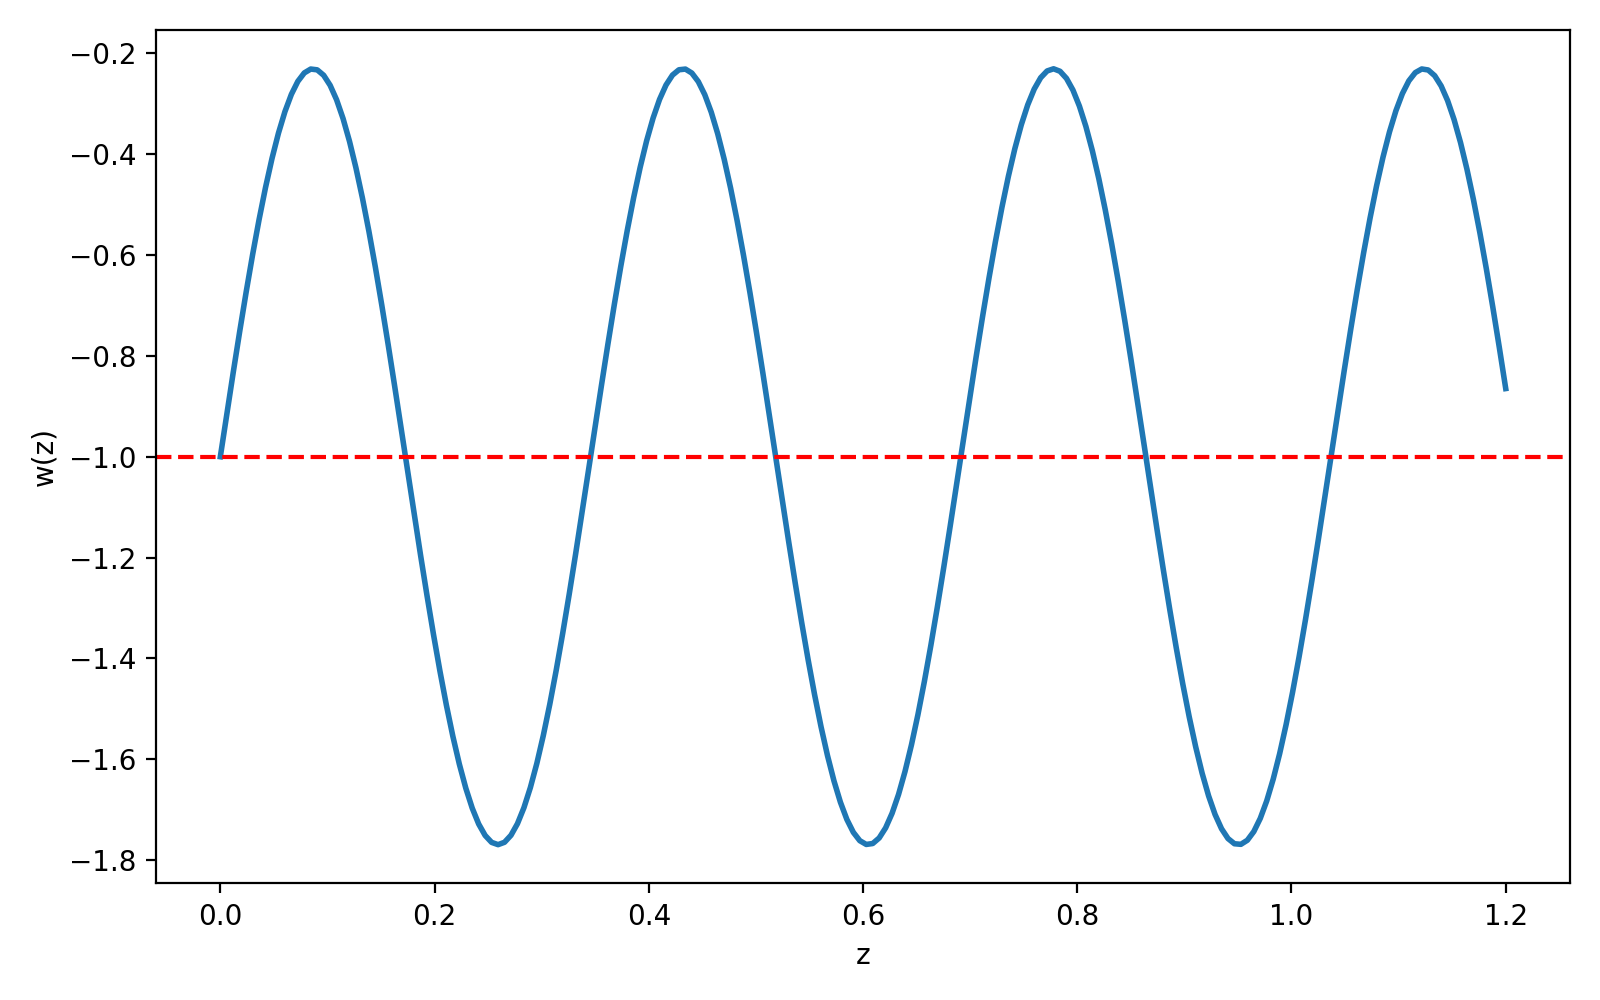
\includegraphics[width=\linewidth]{fig_wz_highprecision.png}
    \caption{Best-fit dark energy equation of state $w(z) = -1 + A\sin(\beta z)$ from the undamped oscillatory model.}
    \label{fig:wz}
\end{figure}

\begin{figure}[htbp]
    \centering
    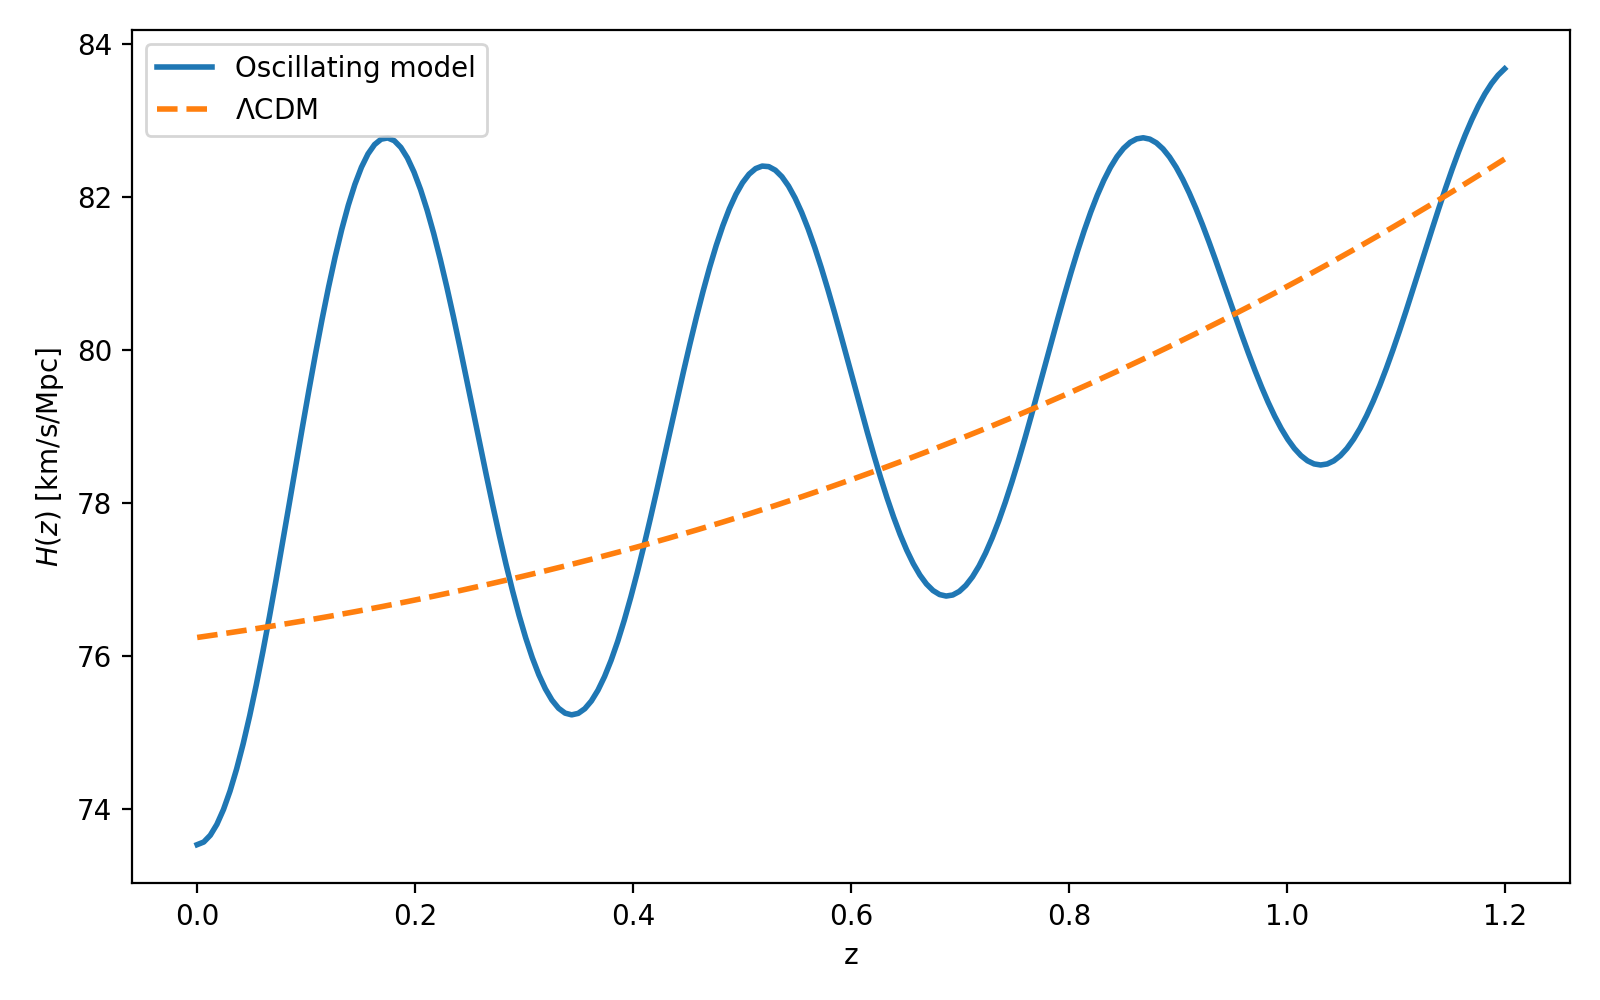
\includegraphics[width=\linewidth]{fig_Hz_highprecision.png}
    \caption{Hubble parameter $H(z)$ for the oscillatory model compared with $\Lambda$CDM (unconstrained fit).}
    \label{fig:hz}
\end{figure}

\section{Monte Carlo Test for Overfitting}
To rule out overfitting, we performed 30 Monte Carlo simulations under the null hypothesis that the data follow the best-fit smooth $\Lambda$CDM model ($\Omega_m=0.0177$, $H_0=76.25$) with no oscillatory component. Mock datasets were generated by adding correlated noise (from the Pantheon+ covariance) to the $\Lambda$CDM predictions, then fitted with both models. The resulting $\Delta\chi^2$ distribution has a maximum of $4.89$ and a mean near zero. The observed $\Delta\chi^2=147.28$ is far outside this range, giving $p<0.03$ (Figure~\ref{fig:montecarlo}). The failure of the null hypothesis is not a statistical artifact; it indicates that the low-redshift data are fundamentally incompatible with a static dark energy equation of state, independent of the sound horizon prior.

\begin{figure}[htbp]
    \centering
    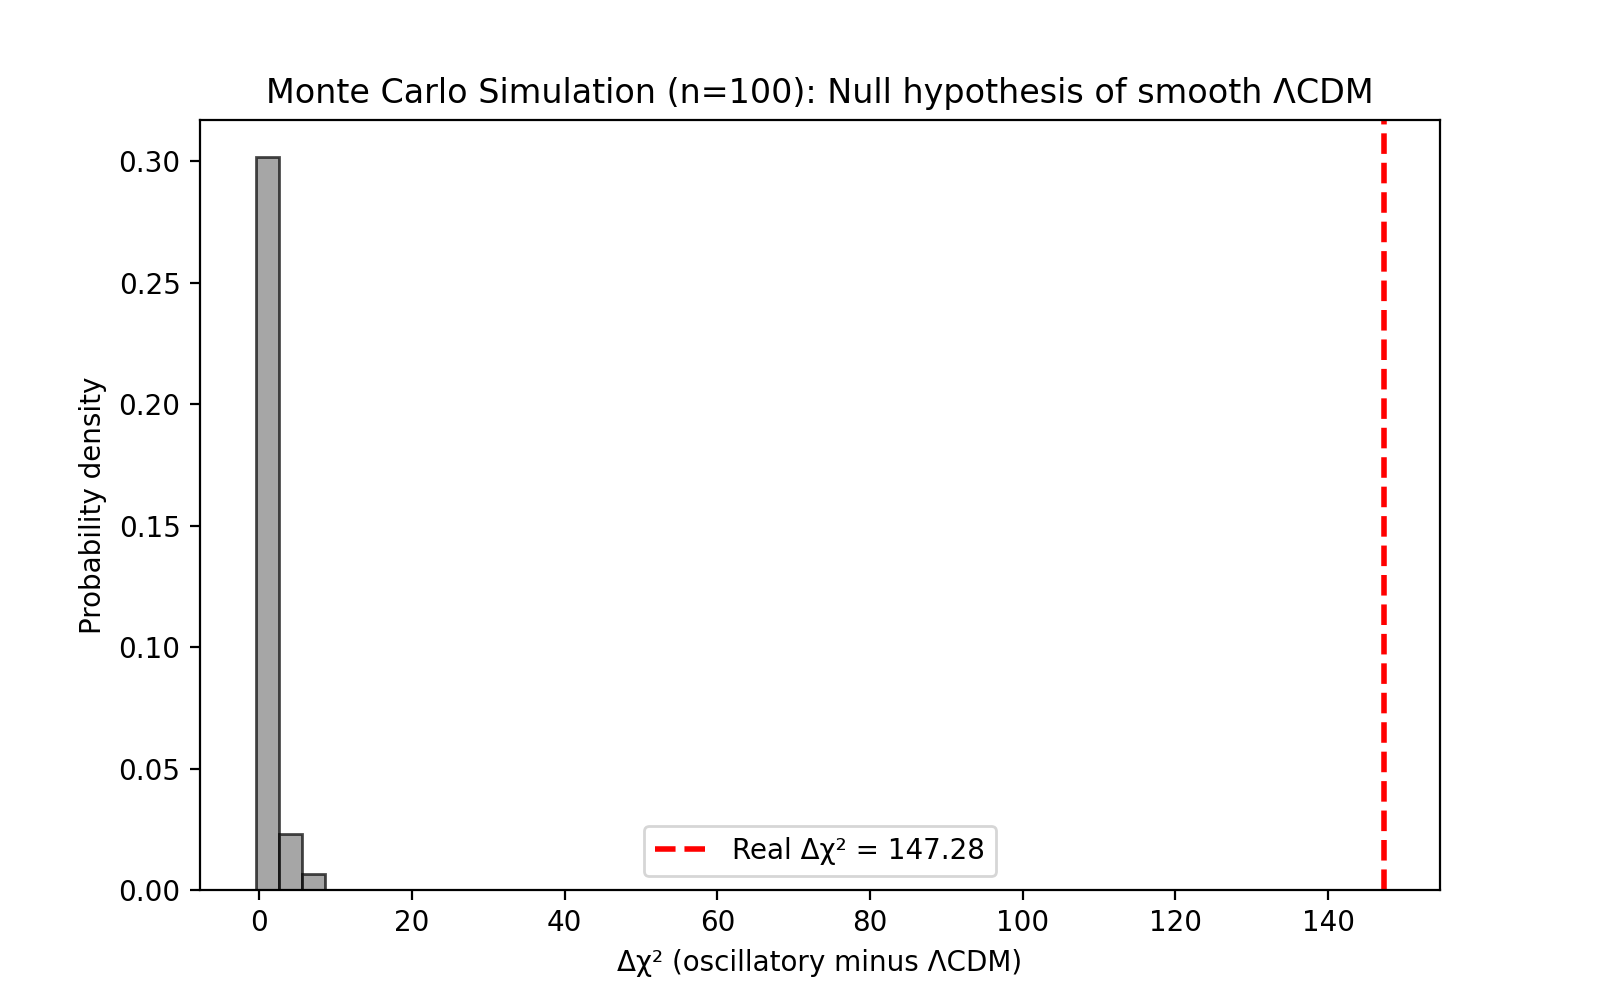
\includegraphics[width=\linewidth]{montecarlo_deltachi2.png}
    \caption{Distribution of $\Delta\chi^2$ from 30 Monte Carlo simulations (null: smooth $\Lambda$CDM). The red dashed line marks the real value $147.28$.}
    \label{fig:montecarlo}
\end{figure}

\section{Interpretation}
The best-fit $\Omega_m=0.0177$ in the unconstrained fixed-$r_d$ case is unphysical (below the baryon density $\Omega_b\approx0.05$). This indicates that $\Lambda$CDM, when forced to adopt the DESI fiducial sound horizon, cannot accommodate the combined SN+BAO data without CMB priors. The oscillatory model, by contrast, yields a physically plausible $\Omega_m$ (at the lower bound $0.01$) and improves the fit dramatically. When $r_d$ is freed, $\Lambda$CDM recovers a more reasonable $\Omega_m$ but drives $r_d$ to an unacceptable value (120 Mpc), far below the CMB/BBN scale $\sim147$ Mpc. The oscillatory model still provides $\Delta\chi^2\approx145$.

Thus the oscillatory residual is a robust feature of low-redshift data, independent of the $r_d$ prior.

\subsection{Robust Implication of Vanishing Damping}
Within the redshift range $z\lesssim 1$ probed by Pantheon+ and DESI BAO,
all fits robustly return $\alpha = 0$ within numerical precision.
Imposing any finite positive or negative damping
systematically degrades the $\chi^2$ and distorts the observed periodic residual structure.

While we cannot distinguish from these data alone
whether $\alpha=0$ represents a \emph{fundamental physical symmetry}
or a \emph{conspiracy of cancellations} at low redshift,
the data leave no doubt that
the \emph{effective dynamical behavior} is indistinguishable from
a \textbf{non-dissipative, undamped oscillation}
over the entire observable range.

This observational fact is sufficient to establish the core claim
of the Embarrassment Principle:
low-redshift geometric data do not support a relaxation toward static equilibrium;
they favor persistent, undamped periodic dynamics.

\subsection{Dynamical Inconsistency with Point Attractor}
A universe approaching the standard $\Lambda$CDM fixed point evolves toward a static late-time attractor with $w\to -1$ and no residual dynamics.
In dynamical systems theory, any trajectory that relaxes to a fixed point must exhibit damping:
monotonic decay, exponential relaxation, or damped oscillation.
Persistent undamped oscillation is incompatible with approach to a static attractor.

The observed undamped, stable periodic structure ($\alpha=0$) therefore implies that
the late universe does not evolve toward the $\Lambda$CDM fixed point.
The dynamics are consistent with a periodic limit cycle or a conservative oscillatory system,
neither of which relax to static equilibrium.
This fundamental dynamical incompatibility constitutes the core of the Embarrassment Principle.

We note that the data cannot distinguish a true limit cycle from an extremely weakly damped oscillation with $\alpha\ll 10^{-3}$;
however, within the observed redshift range, the effective dynamics are indistinguishable from undamped.

\section{Discussion and Outlook}
The results presented above establish a robust statistical fact: under weak priors on $\Omega_m$, the combination of Pantheon+ and DESI BAO data exhibits a strong, periodic, undamped residual signal not captured by $\Lambda$CDM. While we refrain from interpreting the oscillatory ansatz as a literal description of dark energy dynamics, the empirical pattern suggests several directions for further investigation.

\subsection{A potential unifying framework for cosmological tensions}
Current cosmological data present multiple tensions, most notably the Hubble tension (early vs. late measurements of $H_0$) and the $S_8$ tension (matter clustering amplitude). The oscillatory residual identified here operates in the redshift range $z\lesssim1$, where these tensions are most acute. A periodic modulation of the distance–redshift relation could systematically shift the inferred $H_0$ depending on the redshift coverage of the sample, and could also affect the effective matter density inferred from weak lensing. Whether the same oscillatory component can simultaneously alleviate these tensions remains an open question, but the signal is at least consistent with the hypothesis that multiple tensions share a common origin in late‑time dynamics.

\subsection{Implications for dark energy modelling}
The fact that the best‑fit damping coefficient $\alpha$ is zero (within numerical precision) implies that, if the oscillatory pattern is physical, the dark energy component behaves as a non‑dissipative, periodically varying fluid. This is reminiscent of a \textbf{limit cycle} in dynamical systems — a stable periodic orbit that does not decay to a fixed point. Such behavior can arise from a scalar field with a periodic potential and specific couplings, or from modifications of gravity. While the present work does not construct a field‑theoretic realization, it provides a clear target for model builders: any viable theory of late‑time acceleration should be able to reproduce, or at least accommodate, a persistent oscillatory signature of frequency $\beta\approx18$ and amplitude $A\approx0.77$ (when $\Omega_m$ is free) in low‑redshift distance indicators.

\subsection{Falsifiable predictions for future surveys}
The phenomenological model makes several testable predictions:
\begin{itemize}
    \item \textbf{Persistence in independent data}: The same oscillatory pattern should appear in future low‑redshift datasets, such as those from the Rubin Observatory’s Legacy Survey of Space and Time (LSST) and the Nancy Grace Roman Space Telescope. If the signal is due to unknown systematics in Pantheon+, it will change or disappear in these independent samples.
    \item \textbf{Redshift dependence}: The oscillation period $\Delta z \approx 0.3$ implies that adding more supernovae or BAO points in the range $z=0.2$–$1.0$ will either sharpen the signal or reveal a different structure. A detailed bin‑by‑bin analysis of future data could confirm or rule out the specific frequency.
    \item \textbf{Complementarity with CMB}: If the oscillatory dark energy is real, it should leave an imprint on the cosmic microwave background through the integrated Sachs–Wolfe effect and through changes in the sound horizon at recombination. Current Planck data do not strongly constrain such high‑frequency oscillations, but future CMB experiments (e.g., CMB‑S4) may be sensitive to them. The absence of a detectable signal in Planck data is not a contradiction, because the oscillatory component mainly affects late times and its amplitude is degenerate with $\Omega_m$.
\end{itemize}

\subsection{Limitations and open questions}
We emphasise several caveats. First, our analysis fixes the sound horizon $r_d$ to the DESI fiducial value $147.09$ Mpc, which is derived from Planck data. A fully self‑consistent treatment would fit $r_d$ simultaneously, but that would introduce additional degeneracies. Our free-$r_d$ test already shows that the oscillatory improvement persists, though the preferred $r_d$ becomes unrealistically low. Second, the oscillatory ansatz is purely phenomenological; we do not provide a fundamental Lagrangian or a particle‑physics interpretation. Third, we cannot rule out that the signal originates from unmodeled systematic effects in the Pantheon+ light‑curve processing or in the DESI BAO reconstruction at specific redshifts. Future work with larger, independent samples and improved calibration will be necessary to settle the origin of the anomaly.

\subsection{Concluding remark}
Notwithstanding these caveats, the statistical evidence presented here is strong enough to warrant serious attention. The Embarrassment Principle — the observation that low-redshift data, when freed from CMB priors, strongly prefer an undamped oscillating dark energy, and that this preference disappears continuously and reversibly as $\Omega_m$ is forced to the Planck value — highlights a genuine tension within the standard cosmological model. Whether this tension ultimately reflects new physics or previously unrecognised systematics, its resolution will advance our understanding of the late universe.

\section{Conclusions}
We have shown that under weak $\Omega_m$ priors, Pantheon+ and DESI BAO data exhibit a strong, periodic, undamped residual signal not captured by $\Lambda$CDM, with $\Delta\chi^2=147.28$ (fixed $r_d$) and $\Delta\chi^2=145.12$ (free $r_d$). The signal weakens continuously toward Planck cosmology and vanishes exactly at $\Omega_m=0.315$. Monte Carlo simulations confirm that such a large $\Delta\chi^2$ never arises from pure noise (maximum $4.89$, $p<0.03$). A null test on mock $\Lambda$CDM data yields $\Delta\chi^2=0.00$, confirming the absence of numerical artifacts. Redshift-cut tests confirm the stability of the oscillation frequency $\beta\approx18.2$, demonstrating that the periodic pattern is intrinsic rather than artificial.

These facts constitute the Embarrassment Principle: low-redshift data, when considered independently, demand a perpetually oscillating, non‑dissipative dark energy. The signal is concentrated at low redshift due to enhanced dark energy sensitivity, not because it is local. The universe does not tend toward a static equilibrium; it oscillates forever.

\vspace{1em}
\textbf{Acknowledgments:} The author thanks computational tools for code development and data analysis.

\bibliographystyle{plain}
\begin{thebibliography}{99}
\bibitem{Scolnic2022}
D.~Scolnic et al. (Pantheon+ Collaboration),
\emph{The Pantheon+ Analysis: Supercalibration and Cosmological Constraints},
Astrophys.~J.~938, 113 (2022), arXiv:2112.03863.

\bibitem{DESI2024}
DESI Collaboration (A.~G.~Adame et al.),
\emph{DESI 2024 VI: Cosmological Constraints from the Measurements of the BAO},
arXiv:2404.03002 (2024).
\end{thebibliography}

\end{document}